\section{Model Description}
\label{model}

In this section we briefly describe the model introduced in the paper~\cite{voe2007temporal}, 
and focus on more detailed analysis and explanations of the model.

\subsection{The Theta Neuron}


\begin{equation}
\label{theta_model}
	\frac{d\theta}{dt} = (1-\cos \theta) + \alpha I (1 + \cos \theta)
\end{equation}
The theta neuron is described by the differential equation~\ref{theta_model},
where $\theta$ is the \emph{potential} of the neuron  and $I$ is a variable \emph{input current}.
The neuron is said to \emph{fire} every time $\theta$ crosses $\pi$.

Letting $\frac{d\theta}{dt} = 0$, we can derive the stationary points of $\theta$.
When $I > 0$, there is no stationary point, and $\frac{d\theta}{dt}$ is always positive,
while when $I < 0$, there are two stationary points (also called fixed points in the paper): 
An unstable point $\theta_0^+ = \arccos\frac{1 + \alpha I}{1-\alpha I}$ ($\frac{d^2\theta}{dt^2} < 0$ at $\theta_0^+$),
and a stable point $\theta_0^- = -\theta_0^+$ ($\frac{d^2\theta}{dt^2} > 0$ at $\theta_0^-$).
This means that if $I$ keeps a positive constant, a theta neuron will periodically fire,
while if $I$ keeps a negative constant, the theta neuron will fire at most once, and then stay at the stable point $\theta_0^-$.

The paper represents the dynamics of the theta neuron model on a phase circle, as shown in Figure~\ref{phase_circle}.

\begin{figure}
\centering
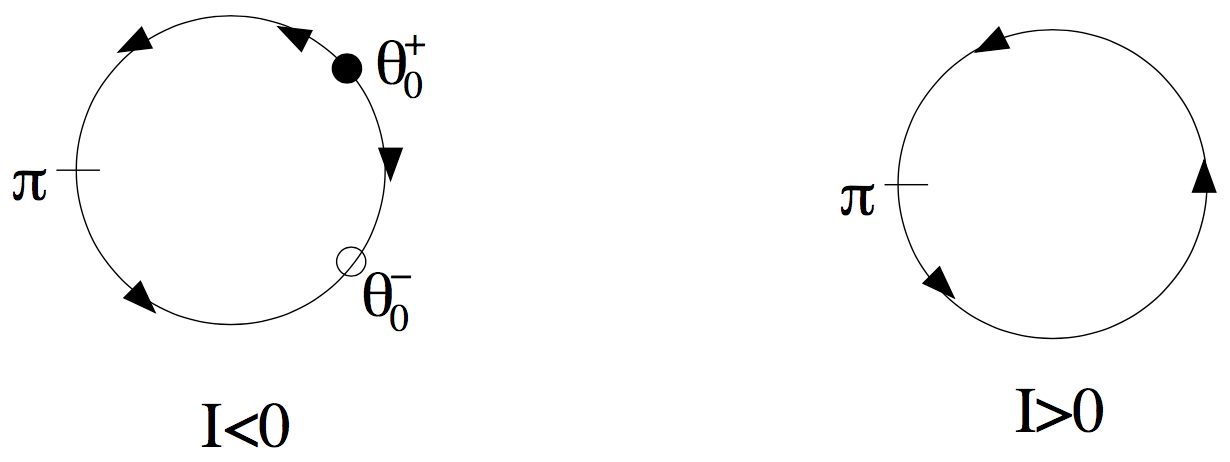
\includegraphics[width=0.6\columnwidth]{phase_circle}
\caption{
\textbf{Phase circle of the theta model.}
The neuron fires every time $\theta$ crosses $\pi$.
For $I < 0$ there are two fixed points: An unstable point $\theta_0^+ = \arccos\frac{1 + \alpha I}{1-\alpha I}$,
and an attractor (stable point) $\theta_0^- = -\theta_0^+$.}
\label{phase_circle}
\end{figure}

\subsection{Synaptic Interactions}

The input current $I$ is the sum of a constant current $I_0$ and transient synaptic currents $I_i(t)$, 
where $i \in 1..N$ indexes the synapses:
\begin{equation}
	I = I_0 + \sum_{i=1}^N I_i(t)
\end{equation}
Synaptic currents are modeled as Diracs: $I_i(t) = w_i\delta(t - t_i)$,
where $t_i$ is the firing time of presynaptic neuron $i$ and $w_i$ the weight of the synapse.

One tricky problem is the calculation of the Dirac delta function $\delta$. 
The author did not mention in the paper how he compute the $\delta(t-t_i)$.
By definition we know % \equation{}
\begin{equation}
\label{dirac}
\delta(t-t_i) = \left\{ \begin{array}{ll}
 A & \textrm{if $t = t_i$}\\
 0 & \textrm{otherwise}
  \end{array} \right.
\end{equation}
but we don't know the choice of $A$.
We were too young too simple and took $1.0$ for $A$, which resulted in mismatch between
the experiment results obtained by us and the author. 
After long time of debugging we find that a larger $A$ is necessary for reproducing the experiment result shown in
the paper.

\subsection{Response Property Analysis of the Theta Model}

We successfully reproduce the simulation results of the relation of the firing time of a theta neuron and the time of arrival of a synaptic current, as shown in Figure~\ref{response}. The results are precisely similar to that shown in the paper.


\begin{figure}
\centering
\subfigure[$I_0 > 0$]{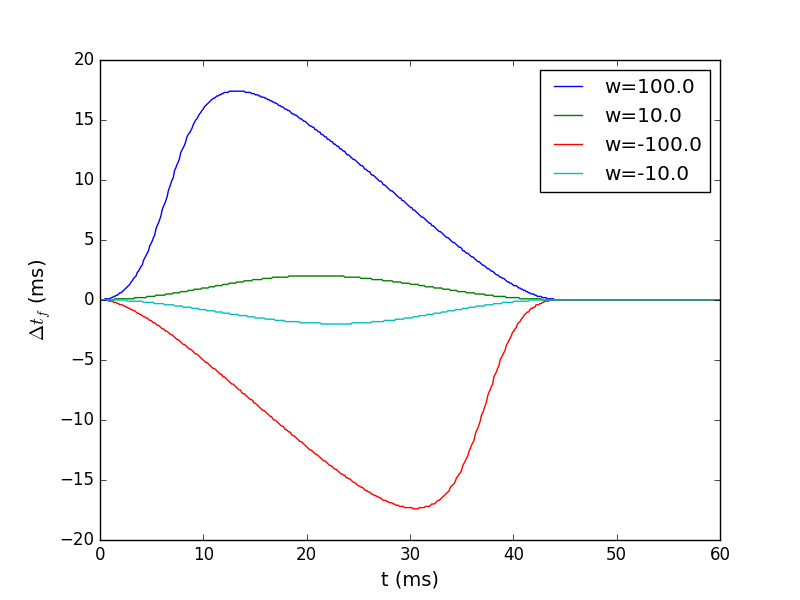
\includegraphics[width=0.98\columnwidth]{response_pos}}
\subfigure[$I_0 < 0$]{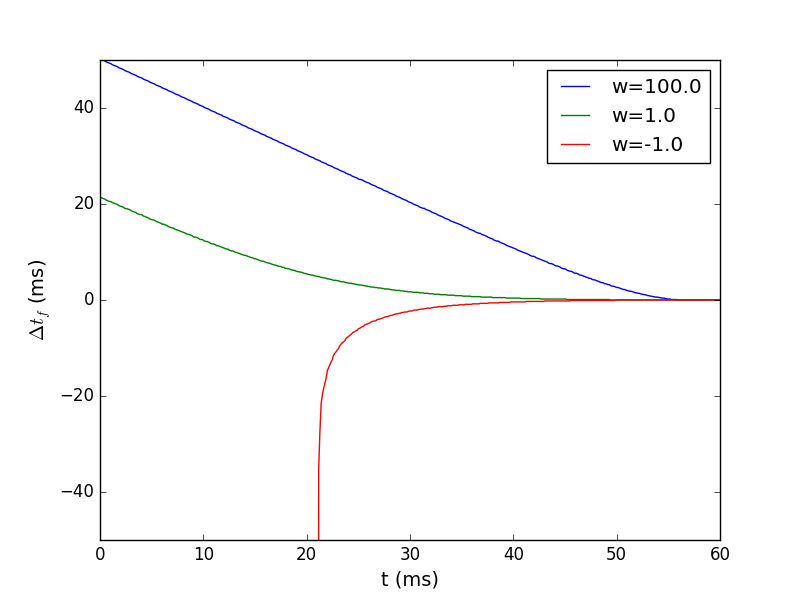
\includegraphics[width=0.98\columnwidth]{response_minus}}
\caption{\textbf{Response properties of the theta model.}
(a) For $I_0 > 0$, the neuron spikes regularly ($I_0 = 0.005$, $\theta(0) = -\pi$). 
The positive curve is called the \emph{Phase Response Curve} (PRC).
(b) Response for $I_0 < 0$.
The initial condition is slightly above the unstable equilibrium point $(I_0 = -0.005, \theta_0 = \theta_0^+ + 0.0001)$.}
\label{response}
\end{figure}

In the time coding model, we view this curve as the transfer function of the neuron; 
it describes how the neuron converts input spike times into output spike times.
Specifically, the curve describes how long the neuron theta will fire \emph{in advance}
(with respect to the firing time without any input presynaptic current) 
when it receives a Dirac current of weight $w$ at time $t$. 


\begin{figure}
\centering
\subfigure[$I_0 > 0$]{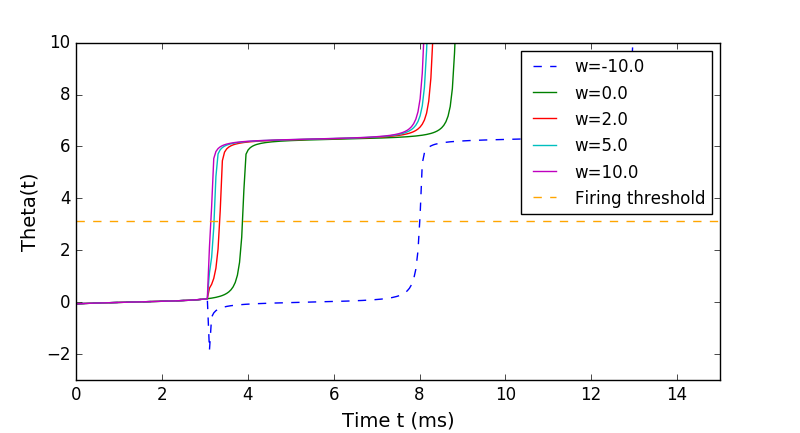
\includegraphics[width=0.98\columnwidth]{theta_t_positive_I}}
\subfigure[$I_0 < 0$]{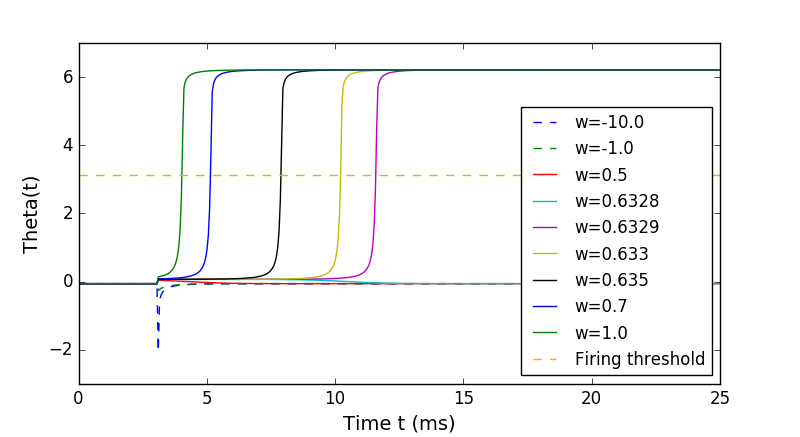
\includegraphics[width=0.98\columnwidth]{theta_t_negtive_I}}
\caption{The relation between $\theta$ and $t$ given different values of $w$. 
There is only one single presynaptic neuron whose firing time is $t_i = 3.0$ ms.
(a) $I_0 = +0.01$. (b) $I_0 = -0.01$. ($\theta_0 = \theta_0^-$ and $\alpha = 0.1$ in both subfigures.)}
\label{theta_t}
\end{figure}

Let's take a closer look at the response properties shown in Figure~\ref{response}.
When $I_0 > 0$, we have seen before that the theta neuron always fires, and from the figure 
we can see that whether it fires earlier or later depends on the sign of the current weight $w$. 
Assume $w$ is positive, we can see that $\Delta t_f$ equals to or is close to $0$ both when $t$ is
small enough and large enough, and $\Delta t_f$ reaches its maximum when $t$ takes a median value.
The reason is two-folded.
On one hand, when $t$ is very small, the input Dirac current comes when $\theta$ is close to the initial
value $\theta(0) = -\pi$, thus $1+\cos \theta$ is close to $0$, and the Dirac current $I$ hardly has any
impact on $\frac {d \theta}{dt}$, let alone impact on $\theta$.
On the other hand, when $t$ is large, the $\theta$ has already been near
to the firing threshold, and the marginal revenue of receiving an input Dirac current at that time is small.
When $t$ is sufficiently large (larger than the firing cycle), the theta neuron fires before the arrival
of the input Dirac current, and thus the firing time is not affected by $t$ anymore.

When $I_0 < 0$, things are more interesting. When $w > 0$, the $\Delta t_f$ is monotone decreasing
with $t$, indicating that the input Dirac current has larger impact when it comes earlier.
When $t$ is sufficiently large and the theta neuron fires first, 
$\Delta t_f$ becomes $0$ for the same reason described above.
However, when $w < 0$ and $t$ is small enough, the theta neuron no longer fires. This is because
when $\theta$ is not too far from the initial value $\theta_0^+$, the input Dirac current, which decreases
$\theta$ when $w < 0$, may take $\theta$ into the range $(-\pi, \theta_0^+)$, ending up with
$\theta = \theta_0^-$. That's why in Figure~\ref{response}(b) the $\Delta t_f$ is unbounded when $t$ is small.


We further show the change of $\theta$ over time by simulations.
We set the arrival time $t$ of the input Dirac current to $3.0$ ms in all simulations.
The results are shown in Figure~\ref{theta_t}.
From Figure~\ref{theta_t}(a) we can see that the theta neuron always fires no matter what the sign
of $w$ is. Positive $w$ makes the theta neuron fires earlier, and vice versa. 
From Figure~\ref{theta_t}(b) we can see that the theta neuron fires when $w=0.6329$, while it never
fires when $w \leq 0.6328$, which means the behavior of the neuron could be very sensitive to the value of
the synapse weight $w$ under certain circumstances.


\subsection{Learning Rule}

The derivation of the learning rule is detailed and clear in the paper. 
We do not repeat the derivation process in this report but highlight some key ideas of it.

Our objective is to learn a set of target firing times $\bar t_s$. That is, we train a set of theta neurons
to fire at the time we would like them to fire. The loss function (cost function) is the mean square error,
denoted by $E = \langle t_s - \bar {t}_s$, where $t_s$ are the actual spike times.
The original work use gradient descent method to optimize $E$, so the derivation of the learning rule
is just computations of partial derivatives.

The firing time $t_s$ is not directly a function of $w_i$, so the author defined a function $F$ 
(see Equation~\ref{F_t}) 
denoting the ``\emph{remaining time}'', i.e., the time that remains before the theta neuron will fire, and thus turned
the calculation of $\frac{\partial t_s}{\partial w_i}$ into calculation of $\frac{\partial F(t)}{\partial w_i}$
($t$ is the current time). 

\begin{equation}
\label{F_t}
	F(t) = \int_{\theta(t)}^\pi \frac{d \theta}{(1-\cos \theta) + \alpha I (1 + \cos \theta)}
\end{equation}

The problem is that $I$ is not continuous, making it unpractical to directly compute $\frac{\partial F(t)}{\partial w_i}$. 
The discontinuity comes from the occurrences of multiple input Dirac currents,
making $I$ and further the integrand a piecewise continuous function.
So the key idea is to break the time domain at $t_i$s ($t_i$ is the time of the $i$-th input Dirac current), 
and compute the derivatives on the intervals.

The final learning rule is described by the following equation:
\begin{equation}
\Delta w_i =
\left\{ \begin{array}{lr}
 -2\eta (t_s - \bar{t}_s) \frac{\partial t_s}{\partial w_i} & \text{if } 0 < - \frac{\partial t_s}{\partial w_i}  < C\\
2\eta (t_s - \bar{t}_s) C & \text{otherwise}
  \end{array} \right.
\end{equation}




